\documentclass{beamer}
\usepackage[utf8]{inputenc}

\usetheme{Madrid}
\usecolortheme{default}
\usepackage{amsmath,amssymb,amsfonts,amsthm}
\usepackage{txfonts}
\usepackage{tkz-euclide}
\usepackage{listings}
\usepackage{adjustbox}
\usepackage{array}
\usepackage{tabularx}
\usepackage{gvv}
\usepackage{lmodern}
\usepackage{circuitikz}
\usepackage{tikz}
\usepackage{graphicx}
\usepackage{multicol}

\setbeamertemplate{page number in head/foot}[totalframenumber]

\usepackage{tcolorbox}
\tcbuselibrary{minted,breakable,xparse,skins}

\definecolor{bg}{gray}{0.95}
\DeclareTCBListing{mintedbox}{O{}m!O{}}{%
  breakable=true,
  listing engine=minted,
  listing only,
  minted language=#2,
  minted style=default,
  minted options={%
    linenos,
    gobble=0,
    breaklines=true,
    breakafter=,,
    fontsize=\small,
    numbersep=8pt,
    #1},
  boxsep=0pt,
  left skip=0pt,
  right skip=0pt,
  left=25pt,
  right=0pt,
  top=3pt,
  bottom=3pt,
  arc=5pt,
  leftrule=0pt,
  rightrule=0pt,
  bottomrule=2pt,
  toprule=2pt,
  colback=bg,
  colframe=orange!70,
  enhanced,
  overlay={%
    \begin{tcbclipinterior}
    \fill[orange!20!white] (frame.south west) rectangle ([xshift=20pt]frame.north west);
    \end{tcbclipinterior}},
  #3,
}
\lstset{
    language=C,
    basicstyle=\ttfamily\small,
    keywordstyle=\color{blue},
    stringstyle=\color{orange},
    commentstyle=\color{green!60!black},
    numbers=left,
    numberstyle=\tiny\color{gray},
    breaklines=true,
    showstringspaces=false,
}

\title 
{9.8.31}
\date{}

\author
{SAMYAK GONDANE - AI25BTECH11029}

\begin{document}

\frame{\titlepage}

\begin{frame}{Question}
Consider a circle with its centre lying on focus of the parabola $y^2 = 2px$ such that it touches the directrix of the parabola. Then a point of intersection of the circle and the parabola is

\begin{multicols}{2}
\begin{enumerate}
    \item $(\frac{p}{2}, p)$ or $(\frac{p}{2}, -p)$
    \item $(\frac{p}{2}, -\frac{p}{2})$
    \item $(-\frac{p}{2}, p)$
    \item $(-\frac{p}{2}, -\frac{p}{2})$
\end{enumerate}
\end{multicols}

\end{frame}

\begin{frame}{Solution}

\textbf{Conic Representation}

Any conic can be expressed as:


\begin{align}
\vec{x}^T V \vec{x} + 2 \vec{u}^T \vec{x} + f = 0
\quad \text{where } \vec{x} = \myvec{x_1 \\ x_2}
\end{align}

\textbf{Parabola: $x_2^2 = 2p x_1$}

Matrix form:

\begin{align}
V_1 = \myvec{0 & 0 \\ 0 & 1}, \quad
\vec{u}_1 = \myvec{-p \\ 0}, \quad
f_1 = 0
\end{align}
\end{frame}


\begin{frame}{Solution}
\textbf{Circle: Center $(\frac{p}{2}, 0)$, Radius $p$}

Expanded form:


\begin{align}
(x_1 - \frac{p}{2})^2 + x_2^2 = p^2
\Rightarrow x_1^2 + x_2^2 - p x_1 - \frac{3p^2}{4} = 0
\end{align}



Matrix form:


\begin{align}
V_2 = \myvec{1 & 0 \\ 0 & 1}, \quad
\vec{u}_2 = \myvec{-\frac{p}{2} \\ 0}, \quad
f_2 = -\frac{3p^2}{4}
\end{align}
\end{frame}


\begin{frame}{Solution}
\textbf{Parametric Line of Intersection}

Using the parametric form of the chord of intersection between the parabola and the circle:


\begin{align}
\vec{x}(\mu) = \vec{h} + \mu \vec{m}
\end{align}


Here, $\vec{h} = \myvec{\frac{p}{2} \\ 0}$ is the center of the circle (also the focus of the parabola), and $\vec{m} = \myvec{0 \\ 1}$ is the direction vector of the vertical chord.
\end{frame}



\begin{frame}{Solution}
Let the line be:


\begin{align}
\vec{x}(\mu) = \vec{h} + \mu \vec{m}
\quad \text{where } \vec{h} = \myvec{\frac{p}{2} \\ 0}, \quad
\vec{m} = \myvec{0 \\ 1}
\end{align}

This gives:

\begin{align}
\vec{x}(\mu) = \myvec{\frac{p}{2} \\ \mu}
\end{align}
\end{frame}



\begin{frame}{Solution}
\textbf{Substitute into Parabola Equation}

We evaluate:


\begin{align}
\vec{x}(\mu)^T V_1 \vec{x}(\mu) + 2 \vec{u}_1^T \vec{x}(\mu) + f_1 = 0
\end{align}

Compute:


\begin{align}
\vec{x}(\mu)^T V_1 \vec{x}(\mu) = \mu^2, \quad
2 \vec{u}_1^T \vec{x}(\mu) = 2(-p)(\frac{p}{2}) = -p^2
\end{align}



So:


\begin{align}
\mu^2 - p^2 = 0 \Rightarrow \mu = \pm p
\end{align}
\end{frame}


\begin{frame}{Solution}
\textbf{Final Intersection Points}

Substitute back:

\begin{align}
\vec{x}(\mu) = \myvec{\frac{p}{2} \\ \pm p}
\end{align}

\textbf{Intersection points:}

\begin{align}
\vec{a}_1 = \myvec{\frac{p}{2} \\ p}, \quad
\vec{a}_2 = \myvec{\frac{p}{2} \\ -p}
\end{align}
\end{frame}


\begin{frame}{Plot}
    \begin{figure}
        \centering
        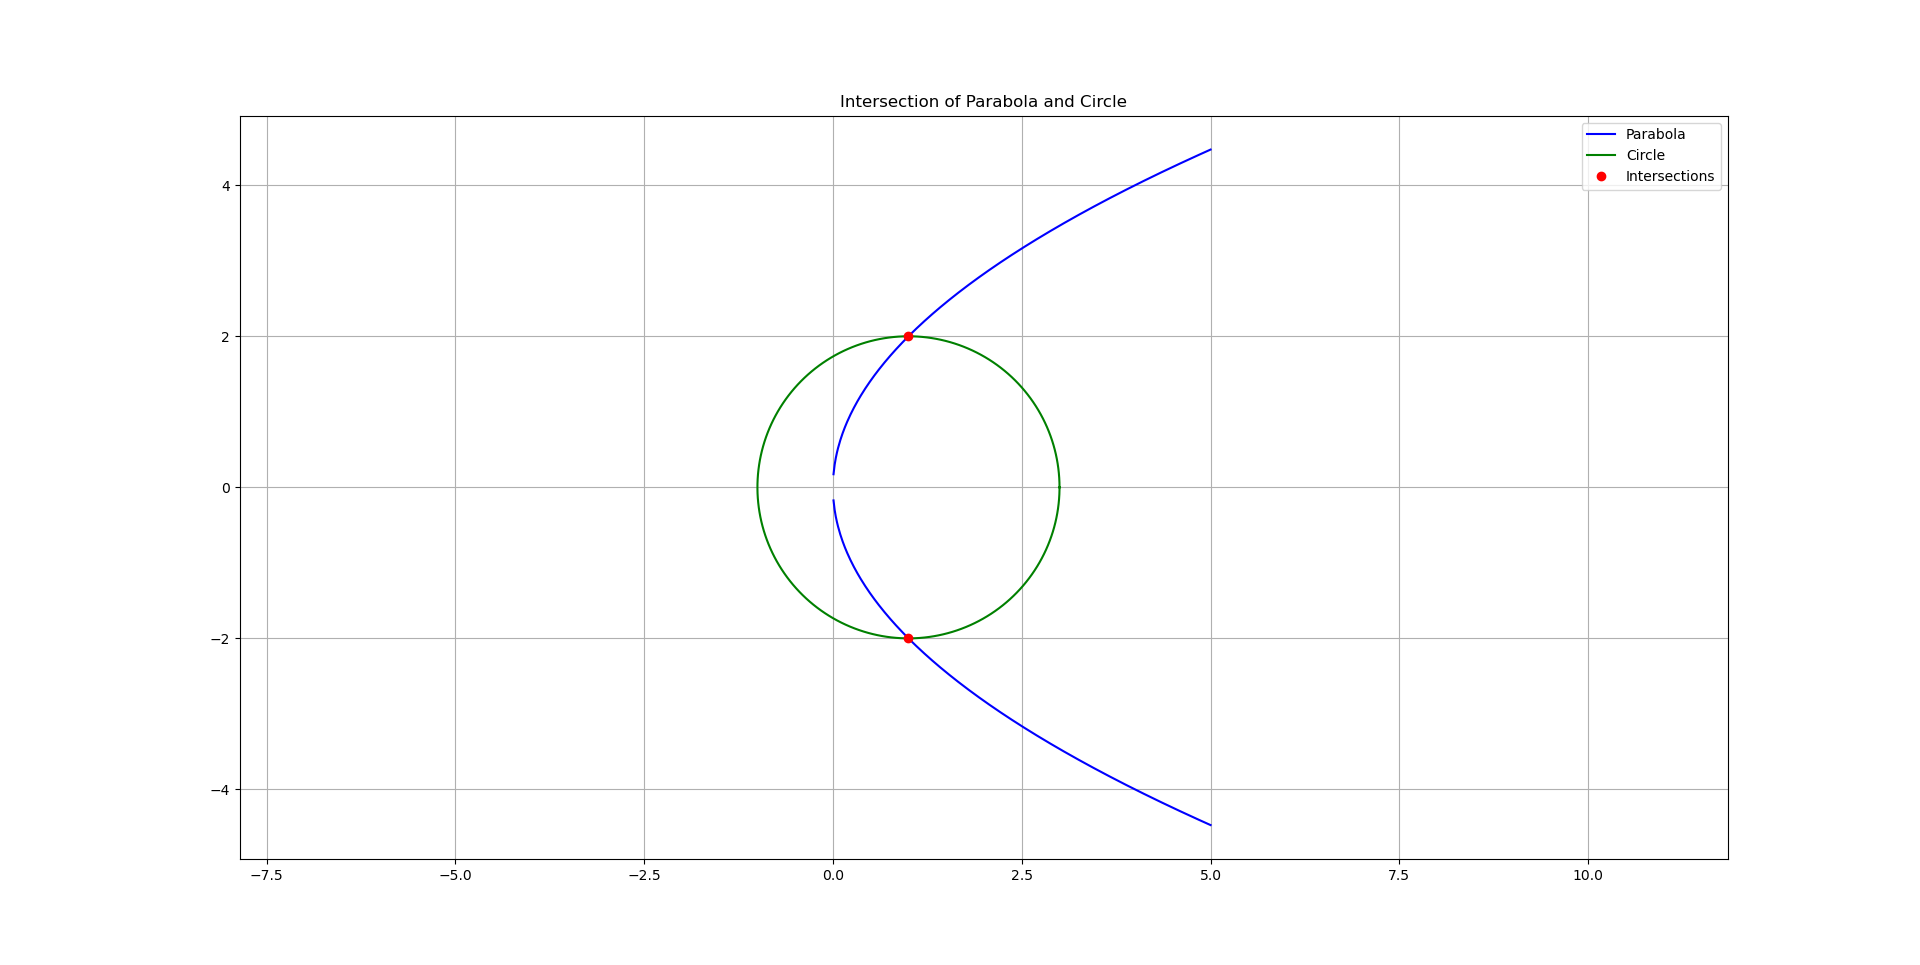
\includegraphics[width=0.8\linewidth]{./figs/Figure_1.png}
        \caption{Caption}
        \label{fig:placeholder}
    \end{figure}
\end{frame}
\end{document}